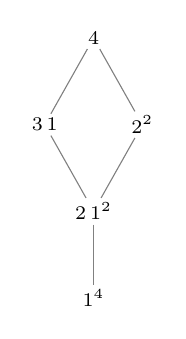
\begin{tikzpicture}[every node/.style={font=\scriptsize,inner sep=1.5pt}]
  \node (p4) at (0.00,3.30) {$4$};
  \node (p3_1) at (-0.62,2.20) {$3\,1$};
  \node (p2_2) at (0.62,2.20) {$2^{2}$};
  \node (p2_1_1) at (0.00,1.10) {$2\,1^{2}$};
  \node (p1_1_1_1) at (0.00,0.00) {$1^{4}$};
  \draw[gray] (p2_1_1) -- (p1_1_1_1);
  \draw[gray] (p2_2) -- (p2_1_1);
  \draw[gray] (p3_1) -- (p2_1_1);
  \draw[gray] (p4) -- (p2_2);
  \draw[gray] (p4) -- (p3_1);
\end{tikzpicture}
